\documentclass{standalone}
\usepackage{tikz}
\usetikzlibrary{patterns, positioning}
\usepackage[sfdefault]{ClearSans} %% option 'sfdefault' activates Clear Sans as the default text font
\usepackage[T1]{fontenc}

\begin{document}
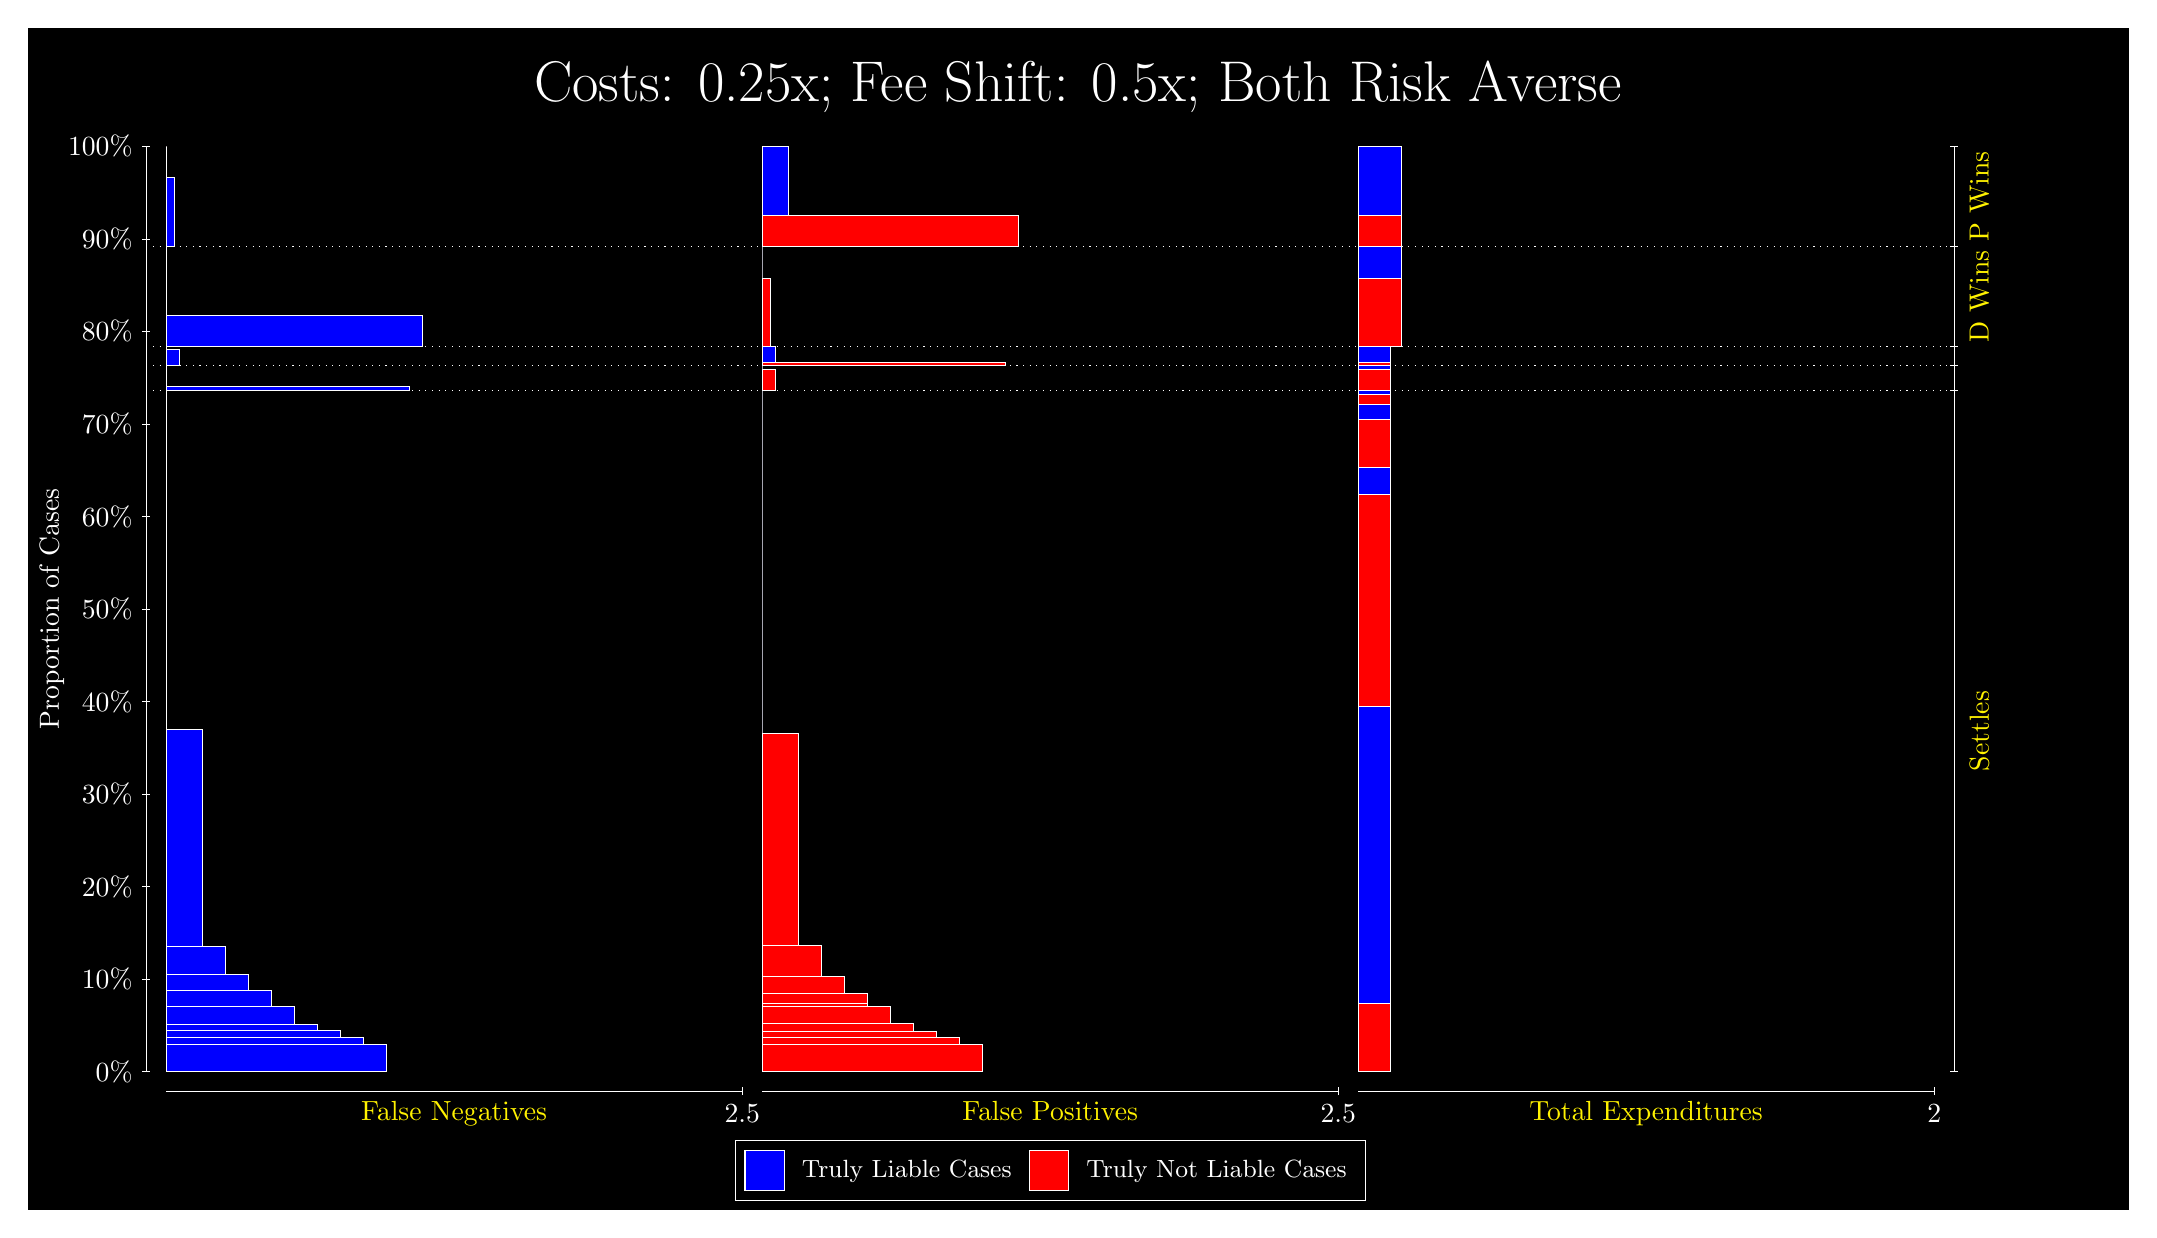
\begin{tikzpicture}
\draw[fill=black] (0,0) rectangle (26.667,15);
\draw[text=white] (0,13.5) rectangle (26.667,15) node[midway] {\huge Costs: 0.25x; Fee Shift: 0.5x; Both Risk Averse};
\draw[white, very thin] (1.5,1.75) -- (1.5,13.5);
\node[rotate=90, text=white, anchor=center] at (0.3, 7.625) {Proportion of Cases};
\draw[white, very thin] (1.45,1.75) -- (1.55,1.75);
\node[text=white, anchor=east] at (1.45, 1.75) {0\%};
\draw[white, very thin] (1.45,2.925) -- (1.55,2.925);
\node[text=white, anchor=east] at (1.45, 2.925) {10\%};
\draw[white, very thin] (1.45,4.1) -- (1.55,4.1);
\node[text=white, anchor=east] at (1.45, 4.1) {20\%};
\draw[white, very thin] (1.45,5.275) -- (1.55,5.275);
\node[text=white, anchor=east] at (1.45, 5.275) {30\%};
\draw[white, very thin] (1.45,6.45) -- (1.55,6.45);
\node[text=white, anchor=east] at (1.45, 6.45) {40\%};
\draw[white, very thin] (1.45,7.625) -- (1.55,7.625);
\node[text=white, anchor=east] at (1.45, 7.625) {50\%};
\draw[white, very thin] (1.45,8.8) -- (1.55,8.8);
\node[text=white, anchor=east] at (1.45, 8.8) {60\%};
\draw[white, very thin] (1.45,9.975) -- (1.55,9.975);
\node[text=white, anchor=east] at (1.45, 9.975) {70\%};
\draw[white, very thin] (1.45,11.15) -- (1.55,11.15);
\node[text=white, anchor=east] at (1.45, 11.15) {80\%};
\draw[white, very thin] (1.45,12.325) -- (1.55,12.325);
\node[text=white, anchor=east] at (1.45, 12.325) {90\%};
\draw[white, very thin] (1.45,13.5) -- (1.55,13.5);
\node[text=white, anchor=east] at (1.45, 13.5) {100\%};

\draw[white, very thin] (24.457,1.75) -- (24.457,13.5);
\draw[white, very thin] (24.407,1.75) -- (24.507,1.75);
\node[anchor=west] at (24.407, 1.75) {};
\draw[white, very thin] (24.407,10.401) -- (24.507,10.401);
\node[anchor=west] at (24.407, 10.401) {};
\draw[white, very thin] (24.407,10.72) -- (24.507,10.72);
\node[anchor=west] at (24.407, 10.72) {};
\draw[white, very thin] (24.407,10.957) -- (24.507,10.957);
\node[anchor=west] at (24.407, 10.957) {};
\draw[white, very thin] (24.407,12.227) -- (24.507,12.227);
\node[anchor=west] at (24.407, 12.227) {};
\draw[white, very thin] (24.407,13.5) -- (24.507,13.5);
\node[anchor=west] at (24.407, 13.5) {};

\draw[white, very thin, fill=blue] (1.75,1.75) rectangle (4.5495,2.0919);
\draw[white, very thin, fill=blue] (1.75,2.0919) rectangle (4.2567,2.1834);
\draw[white, very thin, fill=blue] (1.75,2.1834) rectangle (3.964,2.2765);
\draw[white, very thin, fill=blue] (1.75,2.2765) rectangle (3.6712,2.3545);
\draw[white, very thin, fill=blue] (1.75,2.3545) rectangle (3.3784,2.5782);
\draw[white, very thin, fill=blue] (1.75,2.5782) rectangle (3.0857,2.7875);
\draw[white, very thin, fill=blue] (1.75,2.7875) rectangle (2.7929,2.9866);
\draw[white, very thin, fill=blue] (1.75,2.9866) rectangle (2.5002,3.343);
\draw[white, very thin, fill=blue] (1.75,3.343) rectangle (2.2074,6.1013);
\draw[white, very thin, fill=red] (1.75,6.1013) rectangle (1.75,10.401);
\draw[white, very thin, fill=blue] (1.75,10.401) rectangle (4.8422,10.453);
\draw[white, very thin, fill=red] (1.75,10.453) rectangle (1.75,10.72);
\draw[white, very thin, fill=blue] (1.75,10.72) rectangle (1.9147,10.918);
\draw[white, very thin, fill=red] (1.75,10.918) rectangle (1.75,10.957);
\draw[white, very thin, fill=blue] (1.75,10.957) rectangle (5.0069,11.353);
\draw[white, very thin, fill=red] (1.75,11.353) rectangle (1.75,12.227);
\draw[white, very thin, fill=blue] (1.75,12.227) rectangle (1.8598,13.104);
\draw[white, very thin, fill=red] (1.75,13.104) rectangle (1.75,13.5);
\draw[white, very thin, fill=red] (9.3189,1.75) rectangle (12.118,2.0998);
\draw[white, very thin, fill=red] (9.3189,2.0998) rectangle (11.826,2.1825);
\draw[white, very thin, fill=red] (9.3189,2.1825) rectangle (11.533,2.2659);
\draw[white, very thin, fill=red] (9.3189,2.2659) rectangle (11.24,2.3585);
\draw[white, very thin, fill=red] (9.3189,2.3585) rectangle (10.947,2.5845);
\draw[white, very thin, fill=red] (9.3189,2.5845) rectangle (10.655,2.6159);
\draw[white, very thin, fill=red] (9.3189,2.6159) rectangle (10.655,2.7497);
\draw[white, very thin, fill=red] (9.3189,2.7497) rectangle (10.362,2.9607);
\draw[white, very thin, fill=red] (9.3189,2.9607) rectangle (10.069,3.359);
\draw[white, very thin, fill=red] (9.3189,3.359) rectangle (9.7763,6.0495);
\draw[white, very thin, fill=blue] (9.3189,6.0495) rectangle (9.3189,10.401);
\draw[white, very thin, fill=red] (9.3189,10.401) rectangle (9.4835,10.668);
\draw[white, very thin, fill=blue] (9.3189,10.668) rectangle (9.3189,10.72);
\draw[white, very thin, fill=red] (9.3189,10.72) rectangle (12.411,10.759);
\draw[white, very thin, fill=blue] (9.3189,10.759) rectangle (9.4835,10.957);
\draw[white, very thin, fill=red] (9.3189,10.957) rectangle (9.4287,11.83);
\draw[white, very thin, fill=blue] (9.3189,11.83) rectangle (9.3189,12.227);
\draw[white, very thin, fill=red] (9.3189,12.227) rectangle (12.576,12.623);
\draw[white, very thin, fill=blue] (9.3189,12.623) rectangle (9.6482,13.5);
\draw[white, very thin, fill=red] (16.888,1.75) rectangle (17.299,2.6159);
\draw[white, very thin, fill=blue] (16.888,2.6159) rectangle (17.299,6.3913);
\draw[white, very thin, fill=red] (16.888,6.3913) rectangle (17.299,9.0819);
\draw[white, very thin, fill=blue] (16.888,9.0819) rectangle (17.299,9.4237);
\draw[white, very thin, fill=red] (16.888,9.4237) rectangle (17.299,10.033);
\draw[white, very thin, fill=blue] (16.888,10.033) rectangle (17.299,10.218);
\draw[white, very thin, fill=red] (16.888,10.218) rectangle (17.299,10.351);
\draw[white, very thin, fill=blue] (16.888,10.351) rectangle (17.299,10.401);
\draw[white, very thin, fill=red] (16.888,10.401) rectangle (17.299,10.668);
\draw[white, very thin, fill=blue] (16.888,10.668) rectangle (17.299,10.72);
\draw[white, very thin, fill=red] (16.888,10.72) rectangle (17.299,10.759);
\draw[white, very thin, fill=blue] (16.888,10.759) rectangle (17.299,10.957);
\draw[white, very thin, fill=red] (16.888,10.957) rectangle (17.437,11.83);
\draw[white, very thin, fill=blue] (16.888,11.83) rectangle (17.437,12.227);
\draw[white, very thin, fill=red] (16.888,12.227) rectangle (17.437,12.623);
\draw[white, very thin, fill=blue] (16.888,12.623) rectangle (17.437,13.5);
\draw[white, dotted] (1.5,10.401) -- (24.457,10.401);
\draw[white, dotted] (1.5,10.72) -- (24.457,10.72);
\draw[white, dotted] (1.5,10.957) -- (24.457,10.957);
\draw[white, dotted] (1.5,12.227) -- (24.457,12.227);
\draw[white, very thin] (1.75,1.5) -- (9.0689,1.5);
\node[text=yellow, anchor=north] at (5.4094, 1.5) {False Negatives};
\draw[white, very thin] (9.0689,1.45) -- (9.0689,1.55);
\node[text=white, anchor=north] at (9.0689, 1.45) {2.5};

\draw[white, very thin] (9.3189,1.5) -- (16.638,1.5);
\node[text=yellow, anchor=north] at (12.978, 1.5) {False Positives};
\draw[white, very thin] (16.638,1.45) -- (16.638,1.55);
\node[text=white, anchor=north] at (16.638, 1.45) {2.5};

\draw[white, very thin] (16.888,1.5) -- (24.207,1.5);
\node[text=yellow, anchor=north] at (20.547, 1.5) {Total Expenditures};
\draw[white, very thin] (24.207,1.45) -- (24.207,1.55);
\node[text=white, anchor=north] at (24.207, 1.45) {2};

\node[text=yellow, centered, rotate=90] at (24.777, 6.0754) {Settles};


\node[text=yellow, centered, rotate=90] at (24.777, 11.592) {D Wins};
\node[text=yellow, centered, rotate=90] at (24.777, 12.863) {P Wins};

\draw (12.978300999999998,1.5) node[draw=none] (baseCoordinate) {};
\begin{scope}[align=center]
        \matrix[scale=0.5, draw=white, below=0.5cm of baseCoordinate, nodes={draw}, column sep=0.1cm]{
            \node[rectangle, draw, minimum width=0.5cm, minimum height=0.5cm, fill=blue] {}; &
            \node[draw=none, font=\small, text=white] (B) {Truly Liable Cases}; &
            \node[rectangle, draw, minimum width=0.5cm, minimum height=0.5cm, fill=red] {}; &
            \node[draw=none, font=\small, text=white] (B) {Truly Not Liable Cases}; \\
            };
\end{scope}

\end{tikzpicture}
\end{document}